\documentclass[12pt,a4paper]{article}

\usepackage[utf8]{inputenc}
\usepackage{ctex}
\usepackage{amsmath,amsfonts,amssymb}
\usepackage{abstract,appendix}
\usepackage{makeidx,hyperref}
\usepackage{graphicx,epsfig,subfig}
\usepackage{geometry}
\usepackage{xcolor}

\geometry{scale=0.8}

%\setlength{\lineskip}{\baselineskip}
\setlength{\parskip}{0.5\baselineskip}

\title{Anderson局部化实验报告7}
\author{sis-flag}
\date{\today}

\begin{document}
\maketitle

\section*{原始不等式}

椭圆算子
\begin{align*}
L u = -\nabla (A \nabla u) + b \cdot \nabla u + c u
\end{align*}
算子满足非退化条件,其中$c(x)$是分片常数。

特征值问题
\begin{align*}
L u = \lambda u \quad x \in \Omega \\
\frac{\partial u}{\partial n} + h u = 0 \quad x \in \partial \Omega
\end{align*}
其中$n$是外法方向,$h \geq 0$。

三个右端项问题
\begin{align*}
L w_1 & = 1 \quad x \in \Omega \\
\frac{\partial w_1}{\partial n} & = 0 \quad x \in \partial \Omega \\
w_1(x_0) & = 0
\end{align*}
\begin{align*}
L w_2 & = 1 \quad x \in \Omega \\
\frac{\partial w_2}{\partial n} & = 0 \quad x \in \partial \Omega \\
w_2(x_0) & = 1/\alpha
\end{align*}
\begin{align*}
L w_3 & = 1 \quad x \in \Omega \\
\frac{\partial w_3}{\partial n} + h f(w_3) & = 0 \quad x \in \partial \Omega \\
w_3(x_0) & = 0
\end{align*}
其中$f(x)$是一个非负的函数。(不知道取成$x/\beta$算不算非负函数。。。)

定理告诉我们,归一化后的特征函数和特征值满足
\begin{align*}
|u(x)| \leq |\lambda| w_1(x) + \alpha w_2(x) + \frac{w_3(x)}{\min_{x \in \overline{\Omega}} f(w_3(x))}
\end{align*}

\section*{简化不等式的尝试}

之前在对称算子的时候,其中的$G$可以取为空集,不知道现在还能不能这样选取。

图\ref{dba}中是某一组参数下$w_1$和$w_2$对比图。可以看出,$\alpha$对landscape的影响很小,把G取成空集应该不会有很大问题。
\begin{figure}[h]
\centering
\subfloat[$w_1$]{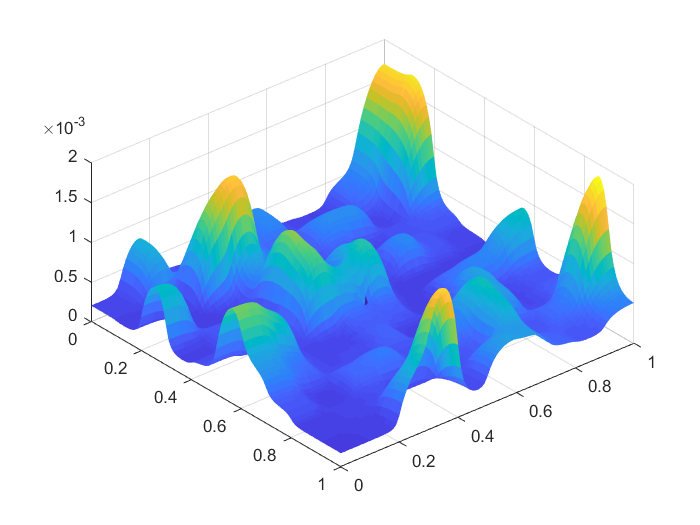
\includegraphics[width=0.3\linewidth]{dba1}}
\subfloat[$w_2$]{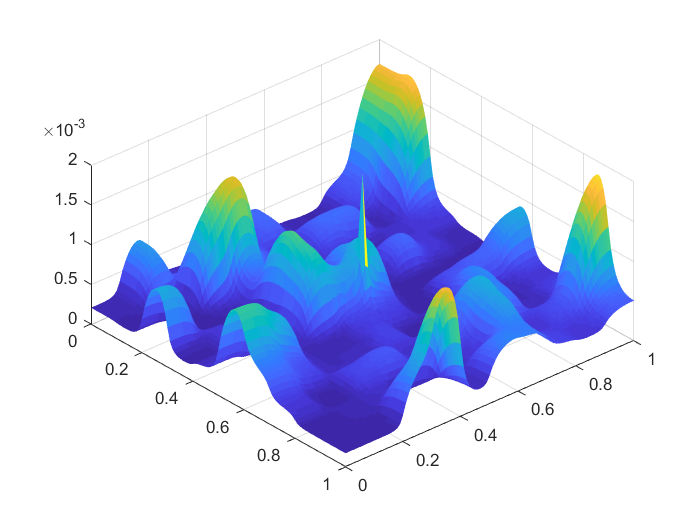
\includegraphics[width=0.3\linewidth]{dba2}}
\caption{模拟结果}
\label{dba}
\end{figure}

由于代码只能计算线性问题,$f$就要取成线性函数$f(w) = \beta w + \gamma$。

在这样的选取下$w_1$和$w_2$完全一样,方程变为
\begin{align*}
L w_1 = L w_3 & = 1 \quad x \in \Omega \\
\frac{\partial w_1}{\partial n} & = 0 \quad x \in \partial \Omega \\
\frac{\partial w_3}{\partial n} + h \beta \ w_3 & = h \gamma \quad x \in \partial \Omega
\end{align*}
特征函数和特征值满足
\begin{align*}
|u(x)| \leq |\lambda| w_1(x) + \frac{w_3(x)}{\beta \min_{x \in \overline{\Omega}} w_3 + \gamma}
\end{align*}

\section*{验证不等式}

一维的情况下,所有的椭圆算子在合适的测度下都是对称算子。这里把$b(x)$选为常数。

选取参数
$$ a(x) = 1; \ b(x) = 10; \ h = 1; \ K = 3000; \ \beta = 10; \ \gamma = 0.1; $$

选取$\beta=1$。相关的解如图\ref{fb1}。第二张图中,红色是$w_2$,蓝色是$w_3$,虽然蓝色的线在边界上翘起来很大,但是它对应的权重很小,landscape并没有很大的变化。第三张图中,实线是landscape,虚线是特征函数的绝对值。这里\textbf{不同的特征函数对应不同的landscape},很难画在一张图里了。
\begin{figure}[h]
\centering
\subfloat[$V(x)$]{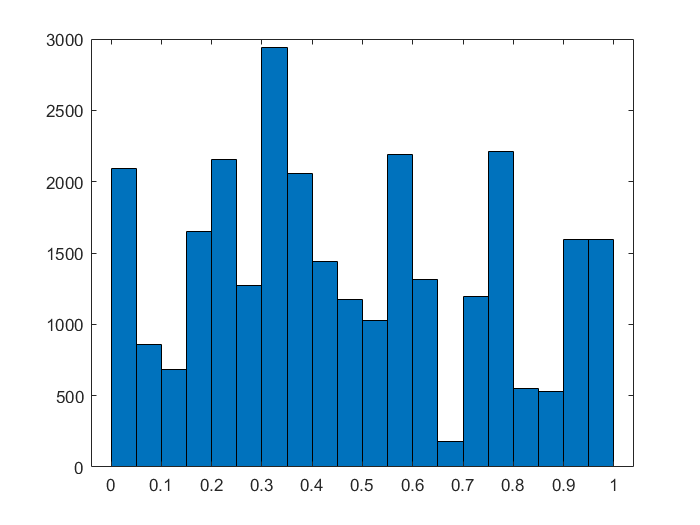
\includegraphics[width=0.3\linewidth]{V1d}}
\subfloat[$w(x)$]{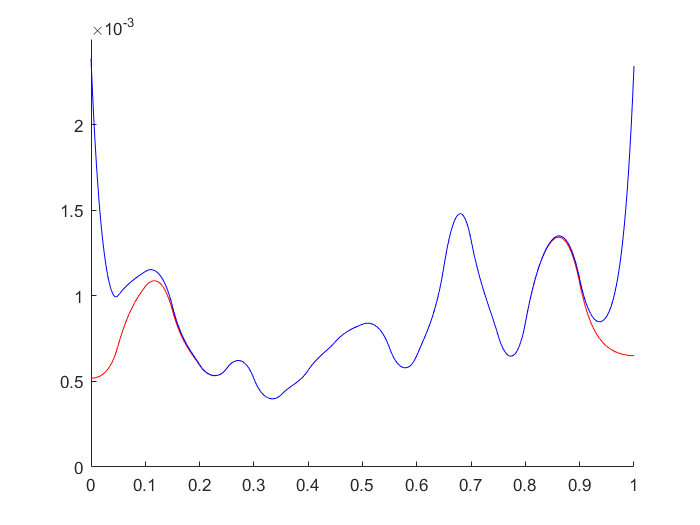
\includegraphics[width=0.3\linewidth]{W1d}}
\subfloat[landscape]{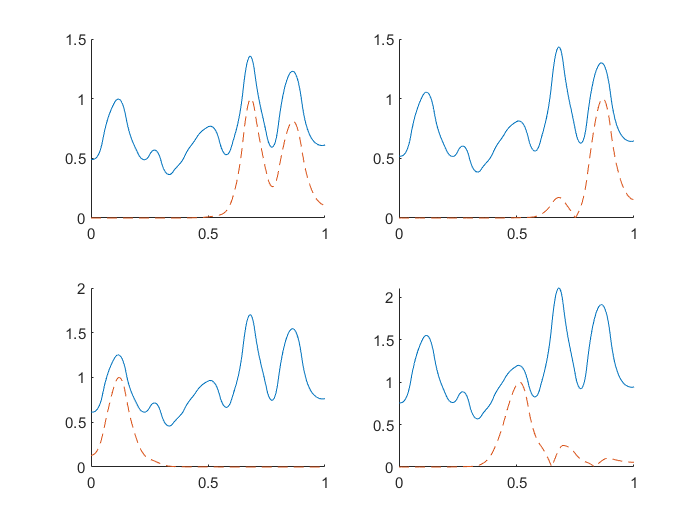
\includegraphics[width=0.3\linewidth]{U1d}}
\caption{模拟结果}
\label{fb1}
\end{figure}

根据经验,这里的参数$\beta, \gamma$对landscape的影响没有那么敏感。此外,landscape的控制效果似乎和K有关。

二维的情况下,参数选取为
$$ a(x) = I; \ b(x) = (10, 20)^T; \ h = 1; \ K = 3000; \ \beta = 10; \ \gamma = 0.1; $$

这里不同的特征函数对应不同的landscape,同样地可以画出很多(大同小异的)valleyline。从图\ref{fb2}和图\ref{fb3}中可以看出,这些landscape可以起到分割特征函数的作用。
\begin{figure}[h]
\centering
\subfloat[$w_1(x)$]{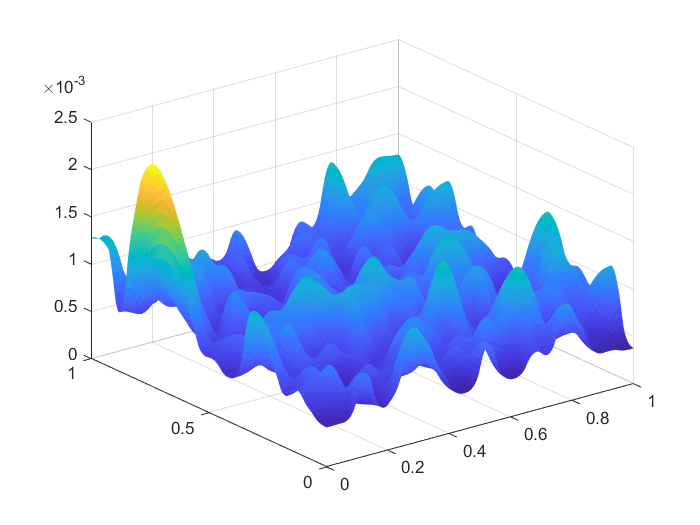
\includegraphics[width=0.3\linewidth]{W12d}}
\subfloat[$w_3(x)$]{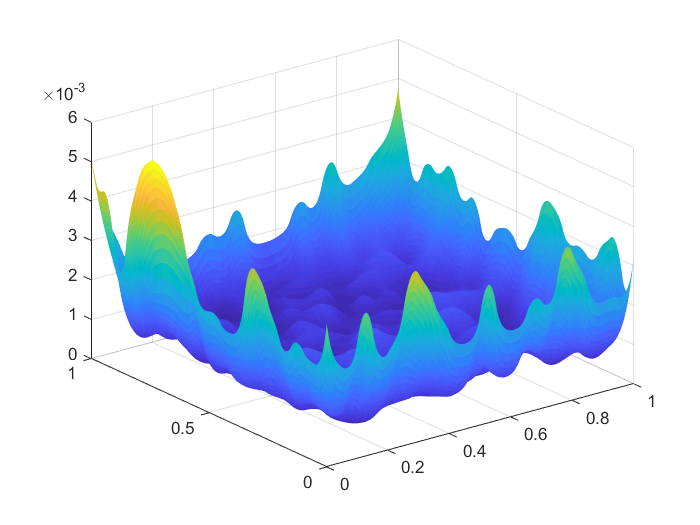
\includegraphics[width=0.3\linewidth]{W32d}}
\caption{landscape(2维)}
\label{fb2}
\end{figure}
\begin{figure}[h]
\centering
\subfloat[$u_1(x)$]{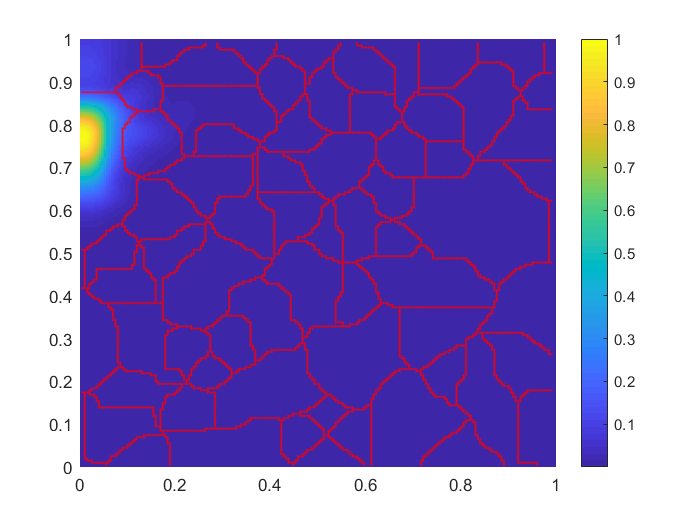
\includegraphics[width=0.3\linewidth]{U12d}}
\subfloat[$u_2(x)$]{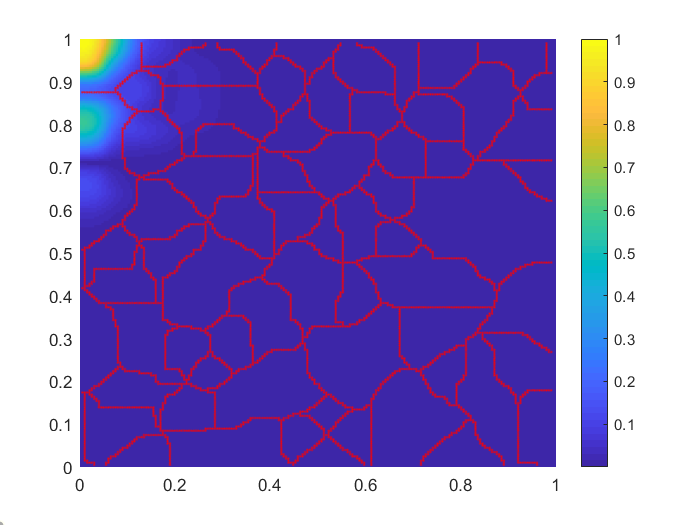
\includegraphics[width=0.3\linewidth]{U22d}}
\subfloat[$u_3(x)$]{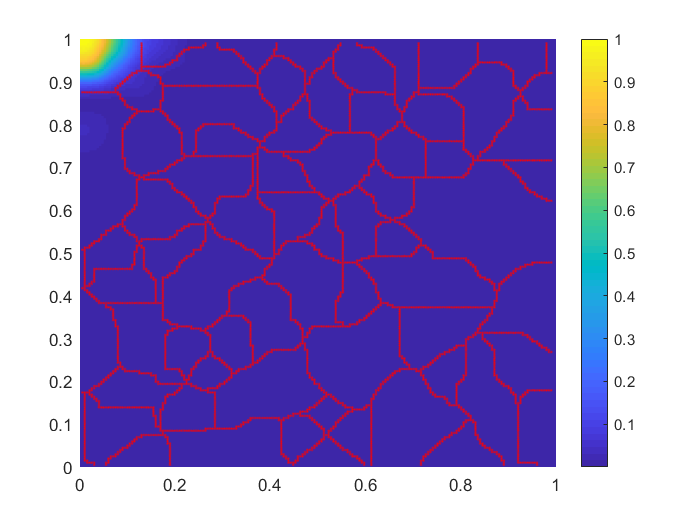
\includegraphics[width=0.3\linewidth]{U32d}}
\caption{特征函数(2维)}
\label{fb3}
\end{figure}

\end{document}